\documentclass{beamer}
\usepackage{amsmath,amsbsy,amsopn,amstext,amsfonts,amssymb}
\usepackage{isomath}
\usepackage{ulem}
%\linespread{1.6}  % double spaces lines
\usepackage{graphicx}
\usepackage{subfigure}
\usepackage{color}
\usepackage{optidef}  % define optimization problems
\usepackage{multicol}  % multiple columns
\usepackage{listings} % for python code
\usepackage{mathrsfs}

\usepackage{polynom}
\newcommand{\adj}{\mathrm{adj}}
\newcommand{\constrainedmin}[3]{
		\begin{mini*}|s|
		{#2}{#1}{}{}
		\addConstraint{#3}
		\end{mini*}
}

\newcommand{\rwbcomment}[1]{{\color{blue}RWB:#1}}
\newcommand{\defeq}{\stackrel{\triangle}{=}}
\newcommand{\abs}[1]{\left|#1\right|}
\newcommand{\norm}[1]{\left\|#1\right\|}
\newcommand{\iprod}[1]{\left<#1\right>}
\newcommand{\ellbf}{\boldsymbol{\ell}}
\newcommand{\nubf}{\boldsymbol{\nu}}
\newcommand{\mubf}{\boldsymbol{\mu}}
\newcommand{\abf}{\mathbf{a}}
\newcommand{\bbf}{\mathbf{b}}
\newcommand{\cbf}{\mathbf{c}}
\newcommand{\dbf}{\mathbf{d}}
\newcommand{\ebf}{\mathbf{e}}
\newcommand{\fbf}{\mathbf{f}}
\newcommand{\gbf}{\mathbf{g}}
\newcommand{\hbf}{\mathbf{h}}
\newcommand{\ibf}{\mathbf{i}}
\newcommand{\jbf}{\mathbf{j}}
\newcommand{\kbf}{\mathbf{k}}
\newcommand{\lbf}{\mathbf{l}}
\newcommand{\mbf}{\mathbf{m}}
\newcommand{\nbf}{\mathbf{n}}
\newcommand{\obf}{\mathbf{o}}
\newcommand{\pbf}{\mathbf{p}}
\newcommand{\qbf}{\mathbf{q}}
\newcommand{\rbf}{\mathbf{r}}
\newcommand{\sbf}{\mathbf{s}}
\newcommand{\tbf}{\mathbf{t}}
\newcommand{\ubf}{\mathbf{u}}
\newcommand{\vbf}{\mathbf{v}}
\newcommand{\wbf}{\mathbf{w}}
\newcommand{\xbf}{\mathbf{x}}
\newcommand{\ybf}{\mathbf{y}}
\newcommand{\zbf}{\mathbf{z}}
\newcommand{\Jbf}{\mathbf{J}}
\newcommand{\Acal}{\mathcal{A}}
\newcommand{\Bcal}{\mathcal{B}}
\newcommand{\Lcal}{\mathcal{L}}
\newcommand{\Ncal}{\mathcal{N}}
\newcommand{\Rcal}{\mathcal{R}}
\definecolor{darkolivegreen}{rgb}{0.33, 0.42, 0.18}

\makeatletter
\newenvironment<>{proofstart}[1][\proofname]{%
    \par
    \def\insertproofname{#1\@addpunct{.}}%
    \usebeamertemplate{proof begin}#2}
  {\usebeamertemplate{proof end}}
\newenvironment<>{proofcont}{%
  \setbeamertemplate{proof begin}{\begin{block}{}}
    \par
    \usebeamertemplate{proof begin}}
  {\usebeamertemplate{proof end}}
\newenvironment<>{proofend}{%
    \par
    \pushQED{\qed}
    \setbeamertemplate{proof begin}{\begin{block}{}}
    \usebeamertemplate{proof begin}}
  {\popQED\usebeamertemplate{proof end}}
\makeatother

\title{ECEn 671: Mathematics of Signals and Systems \\ 
Moon: Chapter 5.}
\author{Randal W. Beard}
\institute{Brigham Young University}
\date{\today}

\begin{document}

%-------------------------------
\begin{frame}
	\titlepage
\end{frame}

%-------------------------------
\begin{frame}[t]
\frametitle{Table of Contents}
\tableofcontents
\end{frame}

%%%%%%%%%%%%%%%%%%%%%%%%%%%%%%%%%%%%%%%%%%%%%%%%%%%%%%%%%%%%%%%%%
\section{LU Factorization}
\frame{\sectionpage}


%----------------------------------
\begin{frame}\frametitle{LU Factorization}
	\begin{itemize}
		\item 	Suppose that $A \in \mathbb{C}^{n\times n}$ is full rank.  What is a numerically efficient method for computing the solution to $Ax = b$, i.e. $x = A^{-1}b$?
		\item An explicit formula is:
			\[ x = \frac{adj(A)b}{det(A)} \]
			but this requires numerical computation of determinants.
		\item LU factorization is more efficient.
	\end{itemize}
\end{frame}

%----------------------------------
\begin{frame}\frametitle{LU Factorization: Basic Idea}
	\begin{itemize}
		\item Find a permutation matrix $P$, a lower diagonal matrix with ones on the diagonal $L$, and an upper diagonal matrix $U$ such that
			\[ PA = LU.\]
		\item How?  Will illustrate by example:
	\end{itemize}
\end{frame}

%----------------------------------
\begin{frame}\frametitle{LU Factorization: cont.}
	Let 
	\[ 
	A = \begin{pmatrix} 
    		1 & -2 & 3\\
    		-4 & 5 & -6\\
    		7 & -8 & 9
    	\end{pmatrix}
    \]
	The idea is to perform row reductions to get a triangular matrix.  
	\par\noindent{\bf Key Idea:}  Reduce the row with the largest element.
\end{frame}

%----------------------------------
\begin{frame}\frametitle{LU Factorization: cont.}
	First, permute $A$ to get the third row on top:
	\begin{align*}
		P_{13}A &= \underbrace{\begin{pmatrix}
						0 & 0 & 1\\
						0 & 1 & 0\\
						1 & 0 & 0
					\end{pmatrix}}_{P_{13}}
					\begin{pmatrix}
    					1 & -2 & 3\\
    					-4 & 5 & -6\\
    					7 & -8 & 9
    				\end{pmatrix} \\
    			&= \begin{pmatrix}
    					7 & -8 & 9\\
    					-4 & 5 & -6\\
    					1 & -2 & 3
    				\end{pmatrix}
    \end{align*}
	The idea is that you always want to divide by the largest element (in absolute value) in the row to avoid numerical problems.
\end{frame}

%----------------------------------
\begin{frame}\frametitle{LU Factorization: cont.}
	Now zero out the $-4$ and $1$ by multiplying the first row by $+\frac{4}{7}$ and adding to the second row and multiplying the first row by 
	$-\frac{1}{7}$ and adding to the third row:
	\begin{align*}
		E_1 P_{13}A 
		&= 
			\underbrace{\begin{pmatrix}
    			1 & 0 & 0\\
    			\frac{4}{7} & 1 & 0\\
    			\frac{-1}{7} & 0 & 1
  			\end{pmatrix}}_{E_1}
			\begin{pmatrix}
    			7 & -8 & 9\\
    			-4 & 5 & -6\\
    			1 & -2 & 3
  			\end{pmatrix} \\
		&=
			\begin{pmatrix}
    			7 & -8 & 9\\
    			0 & 0.4286 & -5.4286\\
    			0 & -0.8571 & 2.8571
  			\end{pmatrix}
	\end{align*}
\end{frame}

%----------------------------------
\begin{frame}\frametitle{LU Factorization: cont.}
	Now permute (or ``pivot'') to get the largest (in absolute value) number in the second column in the second row:
	\begin{align*}
		P_{23}E_1P_{13}A &= 
			\underbrace{\begin{pmatrix}
    			1 & 0 & 0\\
    			0 & 0 & 1\\
    			0 & 1 & 0
  			\end{pmatrix}}_{P_{23}}
			\begin{pmatrix}
    			7 & -8 & 9\\
    			0 & 0.4286 & -5.4286\\
    			0 & -0.8571 & 2.8571
  			\end{pmatrix} \\
		&=
			\begin{pmatrix}
    			7 & -8 & 9\\
    			0 & -0.8571 & 2.8571\\
    			0 & 0.4286 & -5.4286
  			\end{pmatrix}
	\end{align*}
\end{frame}


%----------------------------------
\begin{frame}\frametitle{LU Factorization: cont.}
	Zero out the $0.4286$ by multiplying the second row by 
	$\frac{0.4286}{0.8571}$ and adding to the third row:
	\begin{align*}
		E_2 P_{23} E_1 P_{13} A 
		&= 
			\underbrace{
				\begin{pmatrix}
    				1 & 0 & 0 \\
    				0 & 1 & 0 \\
    				0 & \frac{0.4286}{0.8571} & 1
  				\end{pmatrix}
  			}_{E_2}
			\begin{pmatrix}
    			7 & -8 & 9\\
    			0 & -0.8571 & 2.8571\\
    			0 & 0.4286 & -5.4286
  			\end{pmatrix} \\
		&=
			\begin{pmatrix}
   				7 & -8 & 9\\
    			0 & -0.8571 & 2.8571\\
    			0 & 0 & -4
  			\end{pmatrix} \\ 
  		&= U 
	\end{align*}
	Therefore
	\begin{align*}
		A &= (E_2P_{23}E_1P_{13})^{-1}U \\
		  &= P_{13}^{-1}E_1^{-1}P_{23}^{-1}E_2^{-1} U 
	\end{align*}
\end{frame}

%----------------------------------
\begin{frame}\frametitle{LU Factorization: cont.}
	Note that if 
 	\(
	E_1 = \begin{pmatrix}
    	1 & 0 & 0\\
    	\frac{4}{7} & 1 & 0\\
    	-\frac{1}{7} & 0 & 1
  		\end{pmatrix},
  	\)
  	then
	\(
	E_1^{-1} = \begin{pmatrix}
    	1 & 0 & 0\\
    	-\frac{4}{7} & 1 & 0\\
    	\frac{1}{7} & 0 & 1
    	\end{pmatrix}
	\) \\
	since 
	\[ 
	\begin{pmatrix}
    	1 & 0 & 0\\
    	\frac{4}{7} & 1 & 0\\
    	-\frac{1}{7} & 0 & 1
    \end{pmatrix}
    \begin{pmatrix}
    	1 & 0 & 0\\
    	-\frac{4}{7} & 1 & 0\\
    	\frac{1}{7} & 0 & 1
    \end{pmatrix}
    =\begin{pmatrix}
    	1 & 0 & 0\\
    	0 & 1 & 0\\
    	0 & 0 & 1
    \end{pmatrix}
	\]
	
	\vfill
	
	So the inverse of any lower diagonal matrix formed by multiplying and adding rows is found by negating the off-diagonal terms.
	
	\vfill

	Therefore $E_1^{-1}$ and $E_2^{-1}$ are easy to compute.
\end{frame}
	
%----------------------------------
\begin{frame}\frametitle{LU Factorization: cont.}
	Also note that for permutation matrices 
	\[
	P_{ij}^{-1} = P_{ji}
	\]
	since 
	\[
	\underbrace{P_{ij}}_{\text{switch $ij$ rows}}
	\underbrace{P_{ij}^{-1}}_{\text{ switch back}} = I.
	\]

	For example
	\[
	\begin{pmatrix}
    	0 & 0 & 1\\
    	0 & 1 & 0\\
    	1 & 0 & 0
	\end{pmatrix}
	\begin{pmatrix}
    	0 & 0 & 1\\
    	0 & 1 & 0\\
    	1 & 0 & 0
	\end{pmatrix}
	=
	\begin{pmatrix}
    	1 & 0 & 0\\
    	0 & 1 & 0\\
    	0 & 0 & 1
	\end{pmatrix}.
	\]
\end{frame}

%----------------------------------
\begin{frame}\frametitle{LU Factorization: cont.}
	So we have $A = VU$
	where 
	\(
	V = P_{13}E_1^{-1}P_{23}E_2^{-1} = 
	\begin{pmatrix}
    	0.1429 & 1 & 0\\
    	-0.5714 & -0.5 & 1\\
    	1 & 0 & 0
  	\end{pmatrix}
	\)
	
	\vfill
		
	Note that $V$ is not lower triangular but
	\begin{align*}
	L &= P_{23}P_{13}V = P_{23}
		\begin{pmatrix}
    		1 & 0 & 0\\
    		-0.5714 & -0.5 & 1\\
    		0.1429 & 1 & 0
  		\end{pmatrix} \\
		&= 
		\begin{pmatrix}
    		1 & 0 & 0\\
    		0.1429 & 1 & 0\\
    		-0.5714 & -0.5 & 1
  		\end{pmatrix}
	\end{align*}
	is, so
	\(
	P_{23}P_{13}A = P_{23}P_{13}VU.
	\)
	Therefore
	\[ 
	PA = LU 
	\]
	where $P = P_{23}P_{13}$.
\end{frame}

%----------------------------------
\begin{frame}\frametitle{LU Factorization: cont.}
	For our example we have
	{\footnotesize
	\[
		\underbrace{
			\begin{pmatrix}
    			0 & 0 & 1\\
    			1 & 0 & 0\\
    			0 & 1 & 0
  			\end{pmatrix}
  		}_{P}
		\underbrace{
			\begin{pmatrix}
    			1 & -2 & 3\\
    			-4 & 5 & -6\\
    			7 & -8 & 9
			\end{pmatrix}
		}_{A}
		= 
		\underbrace{
			\begin{pmatrix}
    			1 & 0 & 0\\
    			0.1429 & 1 & 0\\
    			-0.5714 & -0.5 & 1
			\end{pmatrix}
		}_{L}
		\underbrace{
			\begin{pmatrix}
				7 & -8 & 9\\
    			0 & -0.8571 & 2.8571\\
    			0 & 0 & -4	
			\end{pmatrix}
		}_{U}
	\]
	}
	
	How do we solve the equation $ Ax = b$?

	Suppose 
	\(
		b = \begin{pmatrix} 
				1 \\ 2 \\ 3 
			\end{pmatrix}
	\)

	Note that 
	\[ 
		PAx = Pb 
		    = \begin{pmatrix} 
		    	3 \\ 1 \\ 2 
		      \end{pmatrix}
	\]

	So that
	\[ 
		LUx = Pb. 
	\]

\end{frame}

%----------------------------------
\begin{frame}\frametitle{LU Factorization: cont.}
	Let $y = Ux$ then 
	\begin{align*}
		&  	Ly = Pb \\
		\implies \quad & 
			\begin{pmatrix}
    			1 & 0 & 0\\
    			0.1429 & 1 & 0\\
    			-0.5714 & -0.5 & 1
    		\end{pmatrix}
			\begin{pmatrix} 
				y_1 \\ y_2 \\ y_3 
			\end{pmatrix}
			= 
			\begin{pmatrix} 
				3 \\ 1 \\ 2 
			\end{pmatrix} \\
		\implies \quad & 
			\left\{
				\begin{array}{llr}
					y_1 &= 3\\
					y_2 &= 1 - 0.1429y_1 
						& \quad \text{(easy to solve)}\\
					y_3 &= 2 + 0.5714y_1 + 0.5y_2
				\end{array} 
			\right. \\
		\implies \quad & 
			\left\{
				\begin{array}{llr}
					y_1 &= 3\\
					y_2 &= 0.5741 
						& \quad \text{(easy to solve)} \\
					y_3 &= 4
				\end{array}
			\right.
	\end{align*}
\end{frame}

%----------------------------------
\begin{frame}\frametitle{LU Factorization: cont.}
	Next solve $Ux = y$ for $x$:
	\begin{align*}
		& Ux = y \\
		\implies \quad & 	
		\begin{pmatrix}
    		7 & -8 & 9\\
    		0 & -0.8571 & 2.8571\\
    		0 & 0 & -4
    	\end{pmatrix}
    	\begin{pmatrix}
    		x_1 \\ x_2 \\ x_3	
    	\end{pmatrix}
		= 
		\begin{pmatrix}
			3 \\ 0.5714 \\ 4
		\end{pmatrix} \\
		\implies \quad & 
		\left\{
			\begin{array}{rlr}
				-4x_3 &= 4\\
				-0.8571x_2 &= 0.5714 - 2.8571x_2 
					& \quad \text{(easy to solve)}\\
				7x_1 &= 3 + 8x_2 - x_3		
			\end{array} 
		\right. \\
		\implies \quad & 
		\left\{
			\begin{array}{ll}
				x_1 &= -4\\
				x_2 &= -4\\
				x_3 &= -1		
			\end{array}
		\right.
	\end{align*}	
\end{frame}

%----------------------------------
\begin{frame}[fragile]\frametitle{LU Factorization: cont.}
{\small
In Matlab:
	
\begin{lstlisting}[language=Matlab]
    A = [1, 2, 3; 4, 5, 6; 7, 8, 0];
    [L, U, P] = lu(A)	
\end{lstlisting}

\vfill
	
In Python:

\begin{lstlisting}[language=Python]
    import numpy as np
    import scipy.linalg as linalg
		
    A = np.array([[1, 2, 3], [4, 5, 6], [7, 8, 9]])
    P, L, U = linalg.lu(A)
\end{lstlisting}	
}

\vfill

{\bf Homework problem:}  Write your own custom \texttt{lu} function and compare to the built in \texttt{lu} function on 100 randomly generated matrices.
\end{frame}


%%%%%%%%%%%%%%%%%%%%%%%%%%%%%%%%%%%%%%%%%%%%%%%%%%%%%%%%%%%%%%%%%
\section{Cholesky Factorization}
\frame{\sectionpage}

%----------------------------------
\begin{frame}\frametitle{Square Root of a Matrix}
	\begin{itemize}
		\item If $B = B^H > 0$ then we can compute the ``square root'' of $B$ as $B = QQ^H$ where $Q = B^{\frac{1}{2}}$ is the square root of $B$.
		\item In general, the square root of a matrix is not unique!
	\end{itemize}
	\begin{example}
		Let $B = 
		\begin{pmatrix}
			9 & 0\\
			0 & 0
		\end{pmatrix}$
	
	
		We can write
		\[ 
			B = \begin{pmatrix} 3 \\ 0 \end{pmatrix}\begin{pmatrix} 3 & 0 \end{pmatrix} 
		\]
		and
		\[ 
			B = \begin{pmatrix}
					3 & 0\\
					0 & 0
				\end{pmatrix}
				\begin{pmatrix}
					3 & 0\\
					0 & 0
				\end{pmatrix}
		\]
		So both $Q = \begin{pmatrix} 3 \\ 0 \end{pmatrix}$ and $Q = \begin{pmatrix}
			3 & 0\\
			0 & 0
		\end{pmatrix}$ are square roots of $B$.
	\end{example}
\end{frame}

%----------------------------------
\begin{frame}\frametitle{Cholesky Factorization}

	\begin{definition}
	The \underline{Cholesky factorization} of $B$ is a square lower triangular square root $L \in \mathbb{C}^{n \times n}$ of $B$, where 
	\[ B = LL^H. \] 
	\end{definition}

	\vfill
	
	Note that this can also be written as
	\[ B=U^HU \]
	where $U=L^H$ is upper triangular.
\end{frame}

%----------------------------------
\begin{frame}\frametitle{Cholesky Factorization: Numerical Algorithm}
	Let $B = \begin{pmatrix}
		\alpha & \vbf^H \\
		\vbf & B_1
	\end{pmatrix}$. 
	Then factor $B$ as
	\begin{align*}
		B &= \begin{pmatrix}
			\alpha & \vbf^H\\
			\vbf & B_1
			\end{pmatrix} \\
		&=
			\begin{pmatrix}
				\sqrt{\alpha} & 0\\
				\frac{\vbf}{\sqrt{\alpha}} & I_{n-1}
			\end{pmatrix}
			\begin{pmatrix}
				1 & 0\\
				0 & B_1-\frac{\vbf\vbf^H}{\alpha}
			\end{pmatrix}
			\begin{pmatrix}
				\sqrt{\alpha} & \frac{\vbf^H}{\sqrt{\alpha}}\\
				0 & I_{n-1}
			\end{pmatrix}\\
%		&=
%			\begin{pmatrix}
%				\sqrt{\alpha} & 0\\
%				\frac{V}{\sqrt{\alpha}} & B_1 - \frac{vv^H}{\alpha}
%			\end{pmatrix}
%			\begin{pmatrix}
%				\sqrt{\alpha} & \frac{V^H}{\sqrt{\alpha}}\\
%				0 & I_{n-1}
%			\end{pmatrix} \\
%		&= 
%			\begin{pmatrix}
%				\alpha & V^H\\
%				V & B_1
%			\end{pmatrix}
	\end{align*}
	
\end{frame}

%----------------------------------
\begin{frame}\frametitle{Cholesky Factorization: Numerical Algorithm, cont.}
	(RECURSIVE ALGORITHM) \\
	Now find the Cholesky factorization of $B_1 - \frac{\vbf\vbf^H}{\alpha} \defeq  G_1G_1^H$, so that
	\begin{align*}
		B &= 
			\begin{pmatrix}
				\sqrt{\alpha} & 0\\
				\frac{\vbf}{\sqrt{\alpha}} & I_{n-1}
			\end{pmatrix}
			\begin{pmatrix}
				1 & 0\\
				0 & G_1G_1^H
			\end{pmatrix}
			\begin{pmatrix}
				\sqrt{\alpha} & \frac{\vbf^H}{\sqrt{\alpha}}\\
				0 & I_{n-1}
			\end{pmatrix} \\
		 &=
			\begin{pmatrix}
				\sqrt{\alpha} & 0\\
				\frac{\vbf}{\sqrt{\alpha}} & G_1
			\end{pmatrix}
			\begin{pmatrix}
				\sqrt{\alpha} & \frac{\vbf^H}{\sqrt{\alpha}}\\
				0 & G_1^H
			\end{pmatrix}
	\end{align*}
	which implies that the Cholesky factor is
	\[ 
		L = \begin{pmatrix}
				\sqrt{\alpha} & 0\\
				\frac{\vbf}{\sqrt{\alpha}} & G_1
			\end{pmatrix}.
	\]
\end{frame}

%----------------------------------
\begin{frame}\frametitle{Cholesky Factorization: Example}
	Let 
	\(
		B = \begin{pmatrix} 
				1 & 2 & 4 & 1 \\
				2 & 13 & 17 & 8 \\
				4 & 17 & 29 & 16 \\
				1 & 8 & 16 & 30
 			\end{pmatrix}.
 	\)
 	Then 
 	\[
 		B = \begin{pmatrix}
 				\alpha_1 & \vbf_1^\top \\ 
 				\vbf_1 & B_1
 			\end{pmatrix},
 	\]
 	where
 	\begin{align*}
 		\alpha_1 &= 1 \\
 		\vbf_1 &= \begin{pmatrix} 2 & 4 & 1 \end{pmatrix}^\top \\
 		B_1 &= \begin{pmatrix}
 					13 & 17 & 8 \\
 					17 & 29 & 16 \\
 					8 & 16 & 30	
 				\end{pmatrix}.
 	\end{align*}
\end{frame}

%----------------------------------
\begin{frame}\frametitle{Cholesky Factorization: Example, cont.}
	Therefore
	\begin{align*}
		B &= \begin{pmatrix}
 				\sqrt{\alpha_1} & 0^\top \\ \frac{\vbf_1}{\sqrt{\alpha_1}} & G_1
 			 \end{pmatrix}
 			 \begin{pmatrix}
 				\sqrt{\alpha_1} & \frac{\vbf_1^\top}{\sqrt{\alpha_1}} \\ 0 & G_1^\top
 			 \end{pmatrix} \\
 		&= \begin{pmatrix}
				1 & 0 & 0 & 0 \\
				2 &   &   &   \\
				4 &   & G_1 & \\
				1 &   &   & 
			\end{pmatrix}
			\begin{pmatrix}
				1 & 2 & 4 & 1 \\
				0 &   &   &   \\
				0 &   & G_1^\top & \\
				0 &   &   & 
			\end{pmatrix}
	\end{align*}
	where
	\begin{align*}
		G_1 G_1^\top &= B_1 - \frac{\vbf_1 \vbf_1^\top}{\alpha_1} \\
		&= \begin{pmatrix}
 				13 & 17 & 8 \\
 				17 & 29 & 16 \\
 				8 & 16 & 30	
 			\end{pmatrix}
 			- \frac{1}{1}\begin{pmatrix} 2 \\ 4 \\ 1 \end{pmatrix}
 			  \begin{pmatrix} 2 & 4 & 1 \end{pmatrix} \\
 		&= 	\begin{pmatrix}
 				9 & 9 & 6 \\ 9 & 13 & 12 \\ 6 & 12 & 29
 			\end{pmatrix}.
	\end{align*}
\end{frame}

%----------------------------------
\begin{frame}\frametitle{Cholesky Factorization: Example, cont.}
	Therefore
	\begin{align*}
		G_1 G_1^\top &= \begin{pmatrix}
 				\sqrt{\alpha_2} & 0^\top \\ \frac{\vbf_2}{\sqrt{\alpha_2}} & G_2
 			 \end{pmatrix}
 			 \begin{pmatrix}
 				\sqrt{\alpha_2} & \frac{\vbf_2^\top}{\sqrt{\alpha_2}} \\ 0 & G_2^\top
 			 \end{pmatrix} \\
 		&= \begin{pmatrix}
				3 & 0 & 0  \\
				3 &  &  \\
				2 &   & G_2 
			\end{pmatrix}
			\begin{pmatrix}
				3 & 3 & 2 \\
				0 &  & \\
				0 &   &  G_2^\top 
			\end{pmatrix}
	\end{align*}
	where
	\begin{align*}
		G_2 G_2^\top &= B_2 - \frac{\vbf_2 \vbf_2^\top}{\alpha_2} \\
		&= \begin{pmatrix}
 				13 & 12 \\
 				12 & 29  
 			\end{pmatrix}
 			- \frac{1}{9} \begin{pmatrix} 9 \\ 6 \end{pmatrix}
 			  \begin{pmatrix} 9 & 6 \end{pmatrix} \\
 		&= 	\begin{pmatrix}
 				4 & 6 \\ 6 & 25
 			\end{pmatrix}.
	\end{align*}
\end{frame}

%----------------------------------
\begin{frame}\frametitle{Cholesky Factorization: Example, cont.}
	Therefore
	\begin{align*}
		G_2 G_2^\top &= \begin{pmatrix}
 				\sqrt{\alpha_3} & 0^\top \\ \frac{\vbf_3}{\sqrt{\alpha_3}} & G_3
 			 \end{pmatrix}
 			 \begin{pmatrix}
 				\sqrt{\alpha_3} & \frac{\vbf_3^\top}{\sqrt{\alpha_3}} \\ 0 & G_3^\top
 			 \end{pmatrix} \\
 		&= \begin{pmatrix}
				2 & 0   \\
				3 & G_3 
			\end{pmatrix}
			\begin{pmatrix}
				2 & 3  \\
				0 & G_3^\top 
			\end{pmatrix}
	\end{align*}
	where
	\begin{align*}
		G_3 G_3^\top &= B_3 - \frac{\vbf_3 \vbf_3^\top}{\alpha_3} \\
		&= 25 - \frac{1}{4} 3 \cdot 3 \\
 		&= 	16
	\end{align*}
	Therefore $G_3=4$.
\end{frame}

%----------------------------------
\begin{frame}\frametitle{Cholesky Factorization: Example, cont.}
	Combining gives
	{\footnotesize
		\begin{align*}
		L 	&= \begin{pmatrix}
					1 & 0 & 0 & 0 \\
					2 &   &   &   \\
					4 &   & G_1 & \\
					1 &   &   & 
				\end{pmatrix} \\
		 	&= \begin{pmatrix}
					1 & 0 & 0 & 0 \\
					2 & 3 & 0 & 0  \\
					4 & 3 &  &  \\
					1 & 2 &   & G_2 
				\end{pmatrix} \\
		 	&= \begin{pmatrix}
					1 & 0 & 0 & 0 \\
					2 & 3 & 0 & 0  \\
					4 & 3 & 2 & 0   \\
					1 & 2 & 3 & G_3 
				\end{pmatrix} \\			 						
			&= \begin{pmatrix}
					1 & 0 & 0 & 0\\
					2 & 3 & 0 & 0\\
					4 & 3 & 2 & 0\\
					1 & 2 & 3 & 4
				\end{pmatrix}.
		\end{align*}
	}
\end{frame}

%----------------------------------
\begin{frame}\frametitle{Applications of Cholesky Factorization: Quadratic Forms}

	The quadratic form
	\[ 
		x^H Q x = \norm{x }_Q^2
	\]
	where $Q=Q^H$, can be written as
	\[ 
		x^H Qx = x^H U^H Ux = \norm{Ux }_2^2 
	\]
	where $Q = U^HU = LL^H$
	
	\vfill
	In other words, work with the regular 2-norm as opposed to the $Q$ norm.
\end{frame}

%----------------------------------
\begin{frame}\frametitle{Applications of Cholesky Factorization: Simulating a random vector}

	Suppose you want to generate in Matlab/Simulink/Python/etc. a Gaussian random vector with covariance $R = R^T>0$.
	
	\vfill

	The Matlab \texttt{randn([m,1])} command returns an $m\times 1$ random vector which is normally distributed with zero mean and co-variance $I$ ($\mathcal{N}(0,I)$).  
	
	\vfill
	
	To generate $\mathcal{N}(0,R)$ let $R = LL^T$ and let $z = Lx$ where $x \sim \mathcal{N}(0,I)$. 
	
	\vfill 

	Then 
	\begin{align*}
		& E\{zz^T\} = E\{Lxx^TL^T\} = LE\{xx^T\}L^T = LL^T = R \\
		\Rightarrow & z \sim \mathcal{N}(0,R).
	\end{align*}

\end{frame}

%----------------------------------
\begin{frame}\frametitle{Applications of Cholesky Factorization: Solving normal equations}

	Normal equations are given by
	\[
		R\mathbf{c} = \mathbf{b}
	\]
	where $R=R^H$ is the Grammian and full rank if the data vectors are linearly independent.
	
	\vfill
	
	Let $R = LL^H$, then $LL^H \mathbf{c} = \mathbf{b}$
	
	\vfill

	First solve 
	\[ 
	L \mathbf{y} = \mathbf{b}
	\]
	by forward substitution, and then solve
	\[ 
	L^H \mathbf{c} = \mathbf{y}
	\]
	by backward substitution.
\end{frame}

%----------------------------------
\begin{frame}\frametitle{Applications of Cholesky Factorization: Kalman filtering}
	In Kalman filtering we propagate two items;  The estimate $\hat{x}(k)$ and the error covariance $P(k)$ where $P(k)=P^T(k) > 0$.
	
	\vfill

	If implemented directly, numerical error can cause $P(k)$ to become indefinite introducing large errors into the estimate $\hat{x}(k)$.
	
	\vfill

	To avoid this problem a ``square root'' Kalman filter is usually implemented where $P(k) = L(k)L^T(k)$ and $L(k)$ is propagated instead of $P(k)$.  Then even with numerical errors in $L(k)$, $P(k)$ is still symmetric positive definite.

\end{frame}

%----------------------------------
\begin{frame}[fragile]\frametitle{Cholesky Factorization: cont.}
In Matlab:
	
\begin{lstlisting}[language=Matlab]
L1 = [2, 0, 0; 3, 4, 0; 5, 6, 7];
A = L1 * L1';
L = chol(A)'	
\end{lstlisting}

\vfill
	
In Python:

\begin{lstlisting}[language=Python]
import numpy as np
import scipy.linalg as linalg
		
L1 = np.array([[2, 0, 0], [3, 4, 0], [5, 6, 7]])
A = L1 @ L1.T
L = linalg.cholesky(A)
\end{lstlisting}	

$L$ should equal $L_1$.

\vfill

Note that both Matlab and Python return an upper triangular matrix.

\vfill

{\bf Homework problem:}  Write your own custom \texttt{cholesky} function and compare to the built in \texttt{cholesky} function on 100 randomly generated symmetric matrices.
\end{frame}


%%%%%%%%%%%%%%%%%%%%%%%%%%%%%%%%%%%%%%%%%%%%%%%%%%%%%%%%%%%%%%%%%
\section{QR Factorization}
\frame{\sectionpage}

%----------------------------------
\begin{frame}\frametitle{Unitary and Orthogonal Matrices}
	\begin{definition}
	$Q \in \mathbb{C}^{m\times m}$ is \underline{unitary} if
	\[ 
		Q^HQ = QQ^H = I 
	\]
	Equivalently $Q^{-1} = Q^H$.  \\
	Equivalently, the rows of Q form an orthonormal set. \\
	Equivalently, the columns of Q form an orthonormal set.
	\end{definition}

	\begin{definition}
	$Q \in \mathbb{R}^{m \times m} $ is \underline{orthogonal} if 
	\[ 
		Q^TQ = QQ^T = I.
	\]
	\end{definition}
	
	\vfill
	
	Rotation matrices are examples of orthogonal matrices.
\end{frame}

%----------------------------------
\begin{frame}\frametitle{Hermitian Matrices}
	\begin{definition}
	$Q \in \mathbb{C}^{m \times m}$ is \underline{Hermitian} if $Q^H = Q$
	\end{definition}
	
	\vfill
	
	Hermitian matrices are like real numbers, i.e., $\bar{z} = z$.\\
	Unitary matrices correspond to the unit circle
	\[ |z|^2 = \bar{z}z = 1 \]

	\vfill
	
	Bilinear transformation
	\[ 
		z = \frac{1 + jr}{1 - jr} \text{ maps the real line to the unit circle} 
	\]
	
	For matrices this becomes Cayley's formula
	\[ 
		U = (I+jR)(I-jR)^{-1} 
	\]
	which maps Hermitian (analagous to real \#'s) to unitary matrices (analagous to complex unit circle).
\end{frame}

%----------------------------------
\begin{frame}\frametitle{Unitary Matrices, cont}
	\begin{lemma}[Moon Lemma 5.1]
	Let $Q \in \mathbb{C}^{m \times m}$ then $\norm{Qx }_2 = \norm{x }_2,  \forall x \in \mathbb{C}^m~~~$ iff $Q$ is unitary.
	\end{lemma}
	
	\begin{proof}
		If $Q$ is unitary then
		\[
			\norm{Qx }_2 = \iprod{Qx,Qx }^{\frac{1}{2}} = (x^HQ^HQx)^{\frac{1}{2}} = (x^Hx)^{\frac{1}{2}} = \norm{x }_2 
		\]
		Conversely if $\norm{Qx }_2 = \norm{x }_2, \quad \forall x \in \mathbb{C}^m$ then
		\begin{align*}
			& x^HQ^HQx = x^Hx \qquad \forall x\in \mathbb{C}^m \\
			\iff & x^H(Q^HQ-I)x = 0 \qquad \forall x\in \mathbb{C}^m \\
			\iff & Q^HQ = I.
		\end{align*}
		Therefore $Q$ is unitary.
	\end{proof}
\end{frame}

%----------------------------------
\begin{frame}\frametitle{Unitary Matrices, cont}
	\begin{lemma}[Moon Lemma 5.2]
	If $Y=QX$ where $Q$-unitary then 
	\[ \norm{Y }_F = \norm{X }_F \]
	\end{lemma}
\end{frame}

%----------------------------------
\begin{frame}\frametitle{Unitary Matrices, cont.}
	\begin{lemma}
		If 	$Q_1$ and $Q_2$ are unitary then $Q_2Q_1$ is unitary.
	\end{lemma}
	\begin{proof}
		\[ 
			(Q_2Q_1)^H(Q_2Q_1) 
				= Q_1^HQ_2^HQ_2Q_1 
				= Q_1^HQ_1 
				= I.
		\]
	\end{proof}
\end{frame}


%----------------------------------
\begin{frame}\frametitle{QR - Factorization}
	\begin{definition}
		Let $A \in \mathbb{C}^{m \times n}$.  The QR factorization of $A$ is given by
		\[ 
			A = QR 
		\]
		where $Q \in \mathbb{C}^{m \times m}$ is unitary and $R \in \mathbb{C}^{m\times n}$ is upper triangular.
	\end{definition}
	\begin{lemma}
		Every matrix $A\in\mathbb{C}^{m \times n}$ has a QR factorization.	
	\end{lemma}
\end{frame}

%----------------------------------
\begin{frame}\frametitle{QR - Factorization, cont.}
	\begin{example}
		\begin{align*}
		A &= \begin{pmatrix}
				1 & 2 & 3 & 4\\
				5 & 6 & 7 & 8
			\end{pmatrix} \\
		&= 
			\underbrace{
				\begin{pmatrix}
					-0.1961 & -0.9806 \\
					-0.9806 & 0.1961 
		  		\end{pmatrix}
		  	}_Q
		  	\underbrace{
		  		\begin{pmatrix}
					-5.0090 & -6.2757 & -7.4524 & -8.6291\\
					0 & -0.7845 & -1.5689 & -2.3534
		  		\end{pmatrix}
		  	}_R
		\end{align*}
	\end{example}
		
	\vfill
	
	In Matlab: \\
	\texttt{[Q,R] = qr(A)}
	
	\vfill
	
	In Python: \\
	\texttt{Q, R = scipy.linalg.qr(A)}
\end{frame}

%----------------------------------
\begin{frame}\frametitle{QR - Factorization, cont.}
	\begin{example}
		\begin{align*}
			A &= \begin{pmatrix}
					1 & 5\\
					2 & 6\\
					3 & 7\\
					4 & 8
				\end{pmatrix} \\
			&=  \underbrace{
				\begin{pmatrix}
					-0.1826 & -0.8165 & -0.4001 & -0.3741\\
					-0.3651 & -0.4082 & 0.2546 & 0.797\\
					-0.5477 & 0 & 0.6910 & -0.4717\\
					-0.7303 & 0.4082 & -0.5455 & 0.0488
				\end{pmatrix}}_{Q}
				\underbrace{
				\begin{pmatrix}
					-5.4772 & -12.7\\
					0 & -3.266\\
					0 & 0\\
					0 & 0
				\end{pmatrix}}_{R}
		\end{align*}
	\end{example}	
\end{frame}

%----------------------------------
\begin{frame}\frametitle{Application: Full rank least squares}
	If $A \in \mathbb{C}^{m\times n}$ is full rank and $m > n$, find 
	\[ \hat{x} = \arg\min\norm{Ax-b }_2 \]
	
	\vfill
	
	Recall that the solution is $\hat{x} = (A^HA)^{-1}A^Hb$ but
	\[ \mathcal{K}(A^HA) = (\mathcal{K}(A))^2 \]
	
	Therefore computing the inverse of $A^HA$ with LU or Cholesky factorization may be ill-advised. 
	
	\vfill
	
	Use QR factorization instead.
	
\end{frame}

%----------------------------------
\begin{frame}\frametitle{Application: Full rank least squares, cont.}

	Let $A=QR=Q\begin{bmatrix} R_1 \\ 0 \end{bmatrix}$ where $Q\in\mathbb{C}^{m\times m}$ and $R_1\in\mathbb{C}^{n\times n}$ is upper triangular.
	
	\vfill
	
	Let $Q^H\bbf = \begin{pmatrix}\cbf\\\dbf\end{pmatrix}$ where $\cbf\in\mathbb{C}^n$ and $\dbf\in\mathbb{C}^{m-n}$.
	
	Then 
	\begin{align*}
	 \norm{A\xbf - \bbf }_2^2 &= \norm{QR\xbf - \bbf }_2^2 \\
	&= \norm{Q(R\xbf-Q^H\bbf) }_2^2 \qquad \text{( since $QQ^H = I$)} \\
	&= \norm{\begin{bmatrix} R_1 \\ 0 \end{bmatrix}\xbf - \begin{pmatrix}\cbf\\\dbf\end{pmatrix} }_2^2 \qquad \text{ (by lemma 5.1) }\\
	&= \norm{R_1\xbf - \cbf }_2^2 + \norm{\dbf}_2^2 \qquad \text{ (by definition of 2-norm) }
	\end{align*}
	so $\hat{\xbf} = \arg\min \norm{A\xbf-\bbf }_2^2$ satisfies $R_1\hat{\xbf} = \cbf$ where $\hat{\xbf}$ is easily found by forward-substitution.	
\end{frame}

%----------------------------------
\begin{frame}\frametitle{Application: Full rank least squares, cont.}
	Note that we don't actually need to compute all of $Q$ since $Q^H\bbf = \begin{pmatrix}\cbf\\\dbf\end{pmatrix}$.
	
	Let 
	\[
		Q = \begin{pmatrix} 
				\underset{m\times n}{Q_1} & \underset{m\times (m-n)}{Q_2} 
			\end{pmatrix}
	\]
	then
	\[
		Q^Hb = \begin{pmatrix}
 					Q_1^H \\
 					Q_2^H
 			   \end{pmatrix} \bbf
 			 = \begin{pmatrix}
 					Q_1^H \bbf \\
 					Q_2^H \bbf
 				\end{pmatrix}
 			= \begin{pmatrix}
 				\cbf \\ 
 				\dbf
 			  \end{pmatrix}
	\]
	so $\cbf = Q_1^H\bbf$.
	
	\vfill
	
	Therefore, we only need the first $n$ columns of $Q$.
\end{frame}

%----------------------------------
\begin{frame}\frametitle{QR Factorization and Fundamental Subspaces}

	If $A$ is tall then
	\begin{align*}
		A &= QR \\
  		  &= \begin{pmatrix} 
  		  		Q_1 & Q_2 
  		  	  \end{pmatrix}
  		  	  \begin{pmatrix} 
  		  	  	R_1 \\ \mathbf{0} 
  		  	  \end{pmatrix}	
	\end{align*}

	
	\begin{center}
	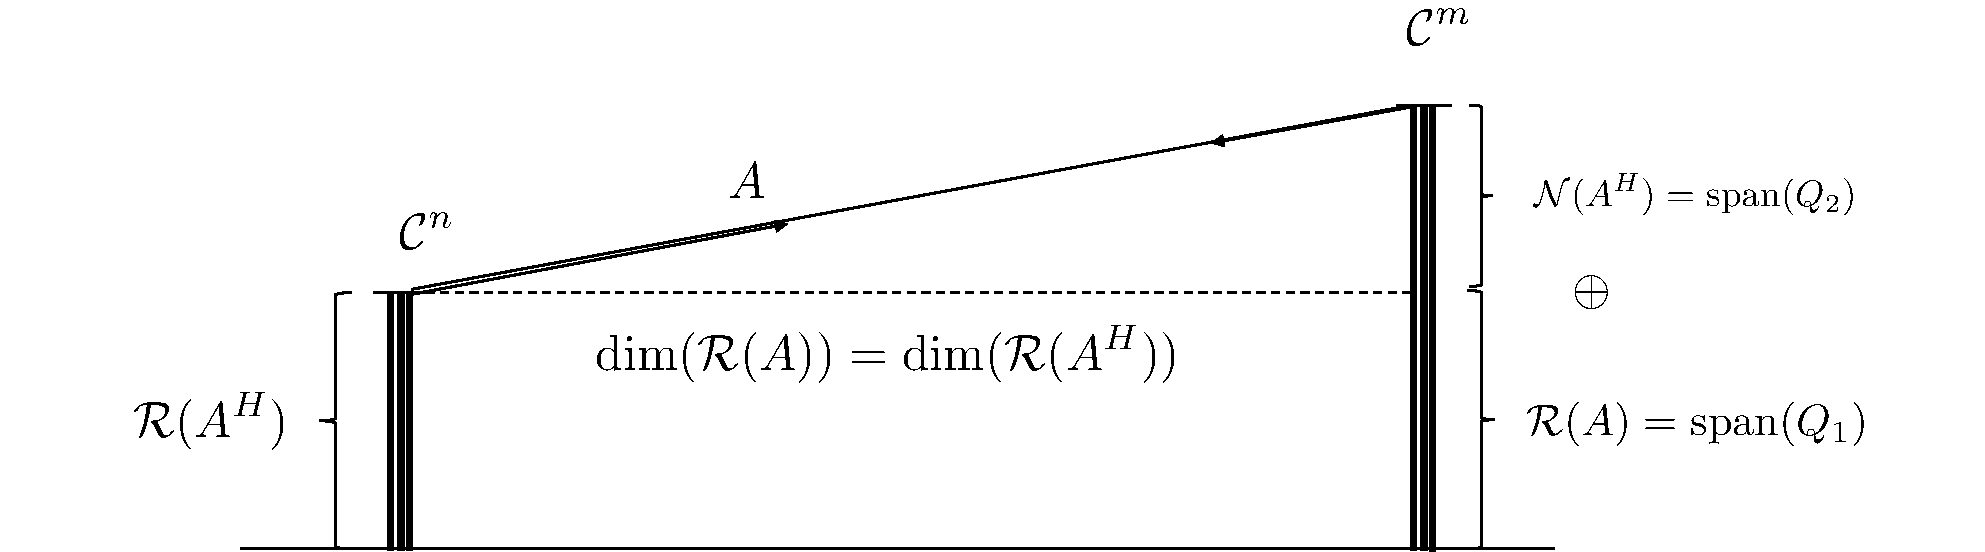
\includegraphics[width=0.9\textwidth]{figures/chap5_qr_subspaces}
	\end{center}

	
\end{frame}




%----------------------------------
\begin{frame}\frametitle{Computational Methods for QR Factorization}

	We will discuss two methods for computing the QR Factorization:

	\begin{itemize}
		\item Given rotation.		
		\item Householder transformation.
	\end{itemize}

\end{frame}

%----------------------------------
\begin{frame}\frametitle{QR Factorization using Given Rotation}
	The basic idea is to diagonalize $A$ one element at at time:
	So find $Q_1$ such that 
		$Q_1A = \begin{pmatrix}x&x\\0&x\\x&x\end{pmatrix}$
		\\
	Then find $Q_2$ such that 
		$Q_2Q_1A = \begin{pmatrix}x&x\\0&x\\0&x\end{pmatrix}$
		\\
	Then find $Q_3$ such that 
		$Q_3Q_2Q_1A = \begin{pmatrix}x&x\\0&x\\0&0\end{pmatrix}$
		\\
	Then 
	\begin{align*}
	A &= (Q_3Q_2Q_1)^{-1}R\\
	&= (Q_3Q_2Q_1)^HR \qquad \text{ (since $(Q_3Q_2Q_1)$ is unitary)}\\
	&= \underbrace{Q_1^HQ_2^HQ_3^H}_{\hat{=}Q}R\\
	&= QR.
	\end{align*}
\end{frame}

%----------------------------------
\begin{frame}\frametitle{QR Factorization using Givens Rotations}
	Consider the $2\times 2$ rotation matrix
	\[ 
		G(\theta) 
			= \begin{pmatrix} 
	    		\cos\theta & \sin\theta \\
	  			-\sin\theta & \cos\theta
	  		  \end{pmatrix}
	\]
	Note that 
	\[
		G^{-1}(\theta) 
			= G^T(\theta) 
			= \begin{pmatrix}
	    		\cos\theta & -\sin\theta\\
	  			+\sin\theta & \cos\theta
	  		  \end{pmatrix}
	\]
	Therefore, $G(\theta)$ is orthogonal and hence unitary.	
\end{frame}

%----------------------------------
\begin{frame}\frametitle{QR Factorization using Givens Rotations}
	Let $x = \begin{pmatrix} r\cos\theta \\ r\sin\theta\end{pmatrix} \in \mathbb{R}^2$:
	\begin{center}
	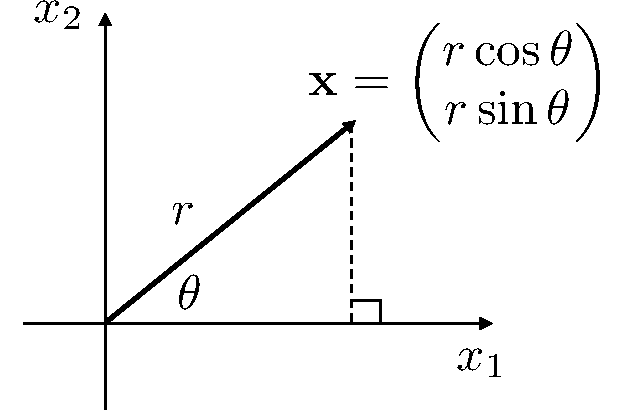
\includegraphics[width=0.5\textwidth]{figures/chap5_givens_1}
	\end{center}
	Then
	\begin{align*} 
		G(\theta)x 
		&= 
			\begin{pmatrix}
	    		\cos\theta & \sin\theta\\
	  			-\sin\theta & \cos\theta
	  		\end{pmatrix}
	  		\begin{pmatrix}
	    		r\cos\theta\\
	  			r\sin\theta
	  		\end{pmatrix} \\
	  	&=
			\begin{pmatrix}
	    		r\cos^2(\theta) + r\sin^2(\theta)\\
	  			-r\sin\theta\cos\theta + r\cos\theta\sin\theta
	  		\end{pmatrix} \\
		&= 
			\begin{pmatrix} r \\ 0 \end{pmatrix}.
	\end{align*}	
\end{frame}

%----------------------------------
\begin{frame}\frametitle{QR Factorization using Givens Rotations}
	Therefore $G(\theta)$ rotated 
	\[
		x = \begin{pmatrix} 
				r\cos\theta \\ 
				r\sin\theta
 			\end{pmatrix}
 	\]
 	to 
 	\[
 		\hat{x} = \begin{pmatrix} r \\ 0 \end{pmatrix}.
 	\]

	\begin{center}
		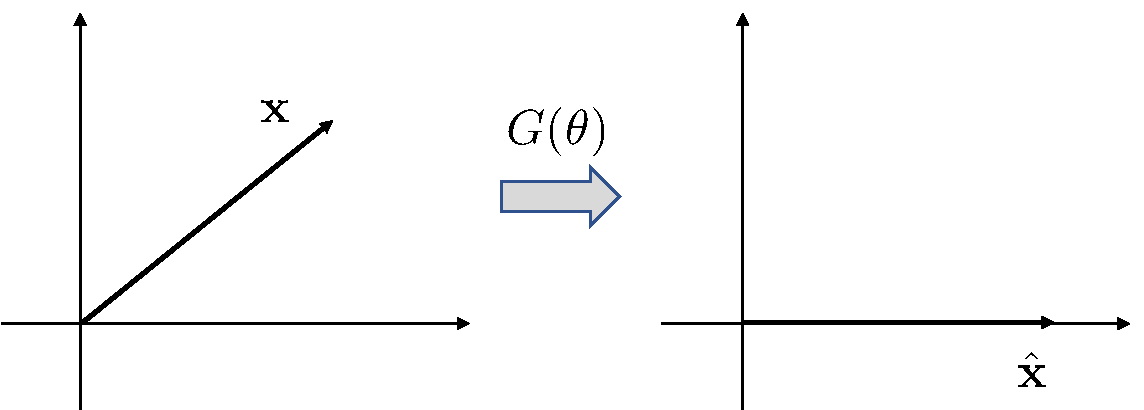
\includegraphics[width=0.5\textwidth]{figures/chap5_givens_2}
	\end{center}
\end{frame}

%----------------------------------
\begin{frame}\frametitle{QR Factorization using Givens Rotations}
	Note that if $x = \begin{pmatrix} x_1 \\ x_2 \end{pmatrix}$ then
	\(
	\theta = \tan^{-1}\left(\frac{x_2}{x_1}\right)
	\)
	and
	\begin{align*}
		\cos\theta &= \cos\left(\tan^{-1}\left(\frac{x_2}{x_1}\right)\right) = \frac{x_1}{\sqrt{x_1^2 + x_2^2}} \\
		\sin\theta &= \sin\left(\tan^{-1}\left(\frac{x_2}{x_1}\right)\right) = \frac{x_2}{\sqrt{x_1^2 + x_2^2}} \\
	\end{align*}
	Therefore
	\[ 
		G_x(\theta) = 
			\begin{pmatrix}
	    		\frac{x_1}{\sqrt{x_1^2 + x_2^2}} & \frac{x_2}{\sqrt{x_1^2 + x_2^2}}\\
	    		-\frac{x_2}{\sqrt{x_1^2 + x_2^2}} & \frac{x_1}{\sqrt{x_1^2 + x_2^2}}
	  		\end{pmatrix}.
	\]
	Note that each term in $G_x(\theta)$ decreases as a result of dividing by $ \frac{1}{\sqrt{x_1^2+x_2^2}} $ so even if $x_1$ and $x_2$ are small, this is numerically stable.

\end{frame}

%----------------------------------
\begin{frame}\frametitle{QR Factorization using Givens Rotations: Example}
	Let
	\[
		A = \begin{pmatrix}
 				1 & 6 & 7 & 12 \\
 				2 & 5 & 8 & 11 \\
 				13 & 4 & 9 & 10
 			\end{pmatrix}
	\]
	Letting $x_1=1$ and $x_2=2$ and 
	\[
		Q_1 = 
			\begin{pmatrix}
 			\frac{x_1}{\sqrt{x_1^2+x_2^2}} & \frac{x_2}{\sqrt{x_1^2+x_2^2}} & 0 \\
 			-\frac{x_2}{\sqrt{x_1^2+x_2^2}} & \frac{x_1}{\sqrt{x_1^2+x_2^2}} & 0 \\
 			0 & 0 & 1
 			\end{pmatrix}
 			=
 			\begin{pmatrix}
				0.4472 & 0.8944 & 0. \\
 				-0.8944 & 0.4472 & 0.\\
 				 0 & 0 & 1
 			\end{pmatrix}
	\]
	gives
	\[
		Q_1 A = 
			\begin{pmatrix}
    			2.2360 & 7.1554 & 10.2859 & 15.2052 \\
				0 & -3.1304 & -2.6832 & -5.8137 \\
				13 & 4 & 9 & 10
			\end{pmatrix}.
	\]
\end{frame}

%----------------------------------
\begin{frame}\frametitle{QR Factorization using Givens Rotations: Example}
	\[
		Q_1 A = 
			\begin{pmatrix}
    			2.2360 & 7.1554 & 10.2859 & 15.2052 \\
				0 & -3.1304 & -2.6832 & -5.8137 \\
				13 & 4 & 9 & 10
			\end{pmatrix}.
	\]
	Letting $x_1=2.2360$ and $x_2=13$ and 
	\[
		Q_2 = 
			\begin{pmatrix}
 			\frac{x_1}{\sqrt{x_1^2+x_2^2}} & 0 & \frac{x_2}{\sqrt{x_1^2+x_2^2}} \\
 			0 & 1 & 0 \\
 			-\frac{x_2}{\sqrt{x_1^2+x_2^2}} & 0 & \frac{x_1}{\sqrt{x_1^2+x_2^2}} 
 			\end{pmatrix}
 			=
 			\begin{pmatrix}
				0.1695 & 0 & 0.9855 \\
				0  & 1 & 0 \\
				-0.9855 & 0 & 0.1695
 			\end{pmatrix}
	\]
	gives
	\[
		Q_2 Q_1 A = 
			\begin{pmatrix}
				13.1909 & 5.1550 & 10.6133 & 12.4328 \\
				0 & -3.1304 & -2.6832 & -5.8137 \\
				0  & -6.3737 & -8.6114 & -13.2900
			\end{pmatrix}.
	\]
\end{frame}

%----------------------------------
\begin{frame}\frametitle{QR Factorization using Givens Rotations: Example}
	\[
		Q_2 Q_1 A = 
			\begin{pmatrix}
				13.1909 & 5.1550 & 10.6133 & 12.4328 \\
				0 & -3.1304 & -2.6832 & -5.8137 \\
				0  & -6.3737 & -8.6114 & -13.2900
			\end{pmatrix}.
	\]
	Letting $x_1=-3.1304$ and $x_2=-6.3737$ and 
	\[
		Q_3 = 
			\begin{pmatrix}
				1 & 0 & 0 \\
	 			0 &\frac{x_1}{\sqrt{x_1^2+x_2^2}} & \frac{x_2}{\sqrt{x_1^2+x_2^2}} \\
 				0 & -\frac{x_2}{\sqrt{x_1^2+x_2^2}} & \frac{x_1}{\sqrt{x_1^2+x_2^2}} 
 			\end{pmatrix}
 			=
 			\begin{pmatrix}
				1 & 0 & 0 \\
				0 & -0.44084797 & -0.8975 \\
				0 & 0.89758179 & -0.4408		
 			\end{pmatrix}
	\]
	gives
	\[
		Q_3 Q_2 Q_1 A = 
			\begin{pmatrix}
				13.1909 & 5.1550 & 10.6133 & 12.4328 & \\
				0 & 7.101 & 8.912 & 14.4918 \\
				0 & 0  & 1.3878 & 0.6405  		
   			\end{pmatrix}.
	\]
\end{frame}

%----------------------------------
\begin{frame}\frametitle{QR Factorization using Givens Rotations: Example}
	Therefore
	{\footnotesize
	\begin{multline*}
	\underbrace{
		\begin{pmatrix}
 			1 & 6 & 7 & 12 \\
 			2 & 5 & 8 & 11 \\
 			13 & 4 & 9 & 10
		\end{pmatrix}
	}_{A}
	\\
	=
	\underbrace{
		\begin{pmatrix}
			0.0967 & 0.9077 & -0.4082 \\
		 	0.4834 & 0.3157 & 0.816 \\
			0.8701 & -0.2763 & 0.4082		
		\end{pmatrix}
	}_{Q}
	\underbrace{
		\begin{pmatrix}
			13.1909 & 5.1550 & 10.6133 & 12.4328 & \\
			0 & 7.101 & 8.912 & 14.4918 \\
			0 & 0  & 1.3878 & 0.6405 
		\end{pmatrix}
	}_R
	\end{multline*}
	}
	where
	\begin{align*}
		Q &= Q_1^H Q_2^H Q_3^H \\
		  &=
		  	\begin{pmatrix}
				0.0758 & 0.7899 & -0.6085 \\
				0.1516 & 0.5940 & 0.7900 \\
				0.9855 & -0.1521 & -0.0747
		  	\end{pmatrix}.
	\end{align*}
\end{frame}

%----------------------------------
\begin{frame}[fragile]\frametitle{QR Factorization using Givens Rotations: Example}
\begin{lstlisting}[language=Python]
import numpy as np

def Q_givens(x1, x2, size, m, n):
    Q = np.eye(size)
    cos_theta = x1 / np.sqrt(x1**2 + x2**2)
    sin_theta = x2 / np.sqrt(x1**2 + x2**2)
    Q[n-1, n-1] = cos_theta
    Q[m-1, m-1] = cos_theta
    Q[m-1, n-1] = -sin_theta
    Q[n-1, m-1] = sin_theta
    return Q

A = np.array([[1, 6, 7, 12],
              [2, 5, 8, 11],
              [13, 4, 9, 10]])
              
\end{lstlisting}
\end{frame}

%----------------------------------
\begin{frame}[fragile]\frametitle{QR Factorization using Givens Rotations: Example}
\begin{lstlisting}[language=Python]

Q1 = Q_givens(x1=1, x2=2, size=3, m=2, n=1)
R1 = Q1 @ A

Q2 = Q_givens(x1=R1[0,0], x2=R1[2,0], size=3, 
              m=3, n=1)
R2 = Q2 @ Q1 @ A

Q3 = Q_givens(x1=R2[1,1], x2=R2[2,1], size=3, 
              m=3, n=2)
R3 = Q3 @ Q2 @ Q1 @ A

Q = Q1.conj().T @ Q2.conj().T @ Q3.conj().T
print("Q=", Q)
print("R=", R3)

\end{lstlisting}
\end{frame}



%----------------------------------
\begin{frame}\frametitle{QR Factorization using Householder Transformation}
	The basic idea is to diagonalize $A$ one column at a time using unitary matrices.  
	\begin{lemma}
		If 	$Q_1$ and $Q_2$ are unitary then $Q_2Q_1$ is unitary.
	\end{lemma}
	\begin{proof}
		\[ 
			(Q_2Q_1)^H(Q_2Q_1) 
				= Q_1^HQ_2^HQ_2Q_1 
				= Q_1^HQ_1 
				= I.
		\]
	\end{proof}
\end{frame}

%----------------------------------
\begin{frame}\frametitle{QR Factorization using Householder Transformation}
	So find $Q_1$ such that 
		$Q_1A = \begin{pmatrix}x&x&x\\0&x&x\\0&x&x\\0&x&x\end{pmatrix}$
		\\
	Then find $Q_2$ such that 
		$Q_2Q_1A = \begin{pmatrix}x&x&x\\0&x&x\\0&0&x\\0&0&x\end{pmatrix}$
		\\
	Then find $Q_3$ such that 
		$Q_3Q_2Q_1A = \begin{pmatrix}x&x&x\\0&x&x\\0&0&x\\0&0&0\end{pmatrix}$
		\\
	Then 
	\begin{align*}
	A &= (Q_3Q_2Q_1)^{-1}R\\
	&= (Q_3Q_2Q_1)^HR \qquad \text{ (since $(Q_3Q_2Q_1)$ is unitary)}\\
	&= \underbrace{Q_1^HQ_2^HQ_3^H}_{\hat{=}Q}R\\
	&= QR.
	\end{align*}
\end{frame}

%----------------------------------
\begin{frame}\frametitle{QR Factorization using Householder Transformation}

	Geometrically what do we want?\\
	
		\begin{center}
		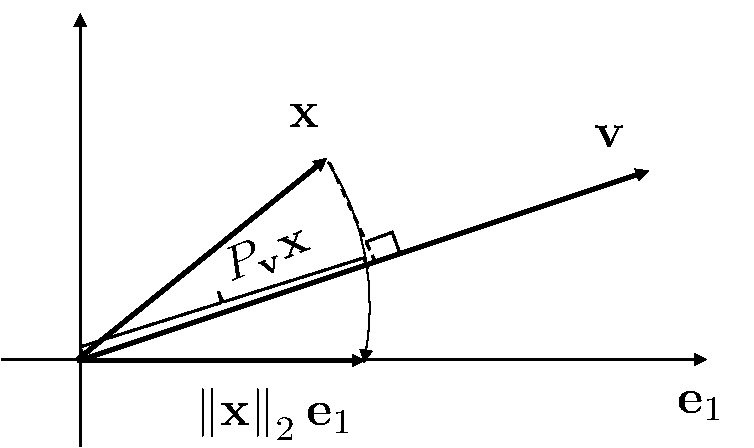
\includegraphics[width=0.5\textwidth]{figures/chap5_householder_1}
		\end{center}
	
	We would like to rotate $x$ down to $e_1$.  This can be thought of as a reflection of $x$ about some vector $v$
	
	\vfill
	
	We need an operator that transforms $x$ to $y=\norm{x }_2e_1$
		
\end{frame}

%----------------------------------
\begin{frame}\frametitle{QR Factorization using Householder Transformation}

	Let 
	\[
		P_v = \frac{vv^H}{v^Hv}
	\] 
	be the projection matrix that projects onto the vector $v$ and let 
	\[
		P_v^{\perp} = I - P_v
	\]

	\begin{center}
	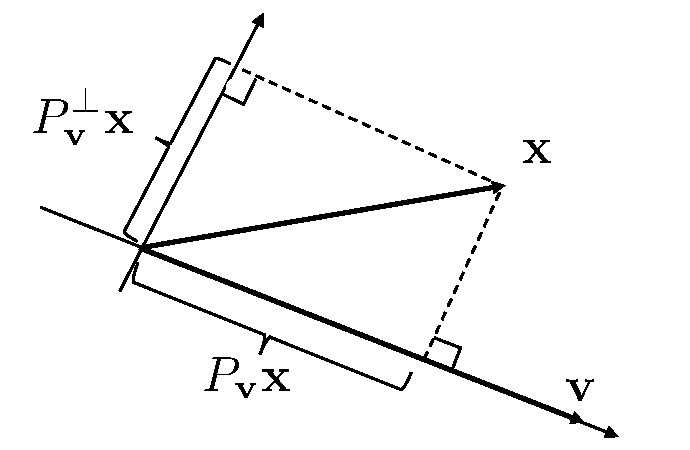
\includegraphics[width=0.5\textwidth]{figures/chap5_householder_2}
	\end{center}
	
\end{frame}

%----------------------------------
\begin{frame}\frametitle{QR Factorization using Householder Transformation}
	The Householder transformation is
	\[ 
		H_v = I - 2P_v 
	\]

	\begin{center}
	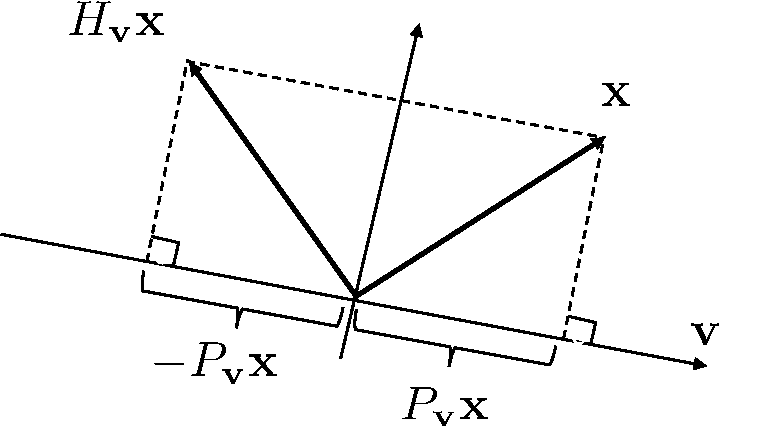
\includegraphics[width=0.5\textwidth]{figures/chap5_householder_3}
	\end{center}

	$H_\vbf \xbf$ reflects $\xbf$ about the vector that is orthogonal to $\vbf$, and in the same hyperplane as both $\xbf$ and $\vbf$.
	
\end{frame}


%----------------------------------
\begin{frame}\frametitle{QR Factorization using Householder Transformation}
	\begin{lemma}
		$H_v$ is unitary.
	\end{lemma}
	\begin{proof}
		\begin{align*}
			H_v^HH_v 
				&= (I - 2P_v^H)^H(I - 2P_v)\\
				&= I - 2P_v - 2P_v + 4P_v^2\\
				&= I - 4P_v + 4P_v \qquad \text{ (since $P_v^2 = P_v$)}\\
				&= I
		\end{align*}
	\end{proof}
\end{frame}

%----------------------------------
\begin{frame}\frametitle{QR Factorization using Householder Transformation}
	\begin{lemma}
		$H_vv = -v$
	\end{lemma}
	\begin{proof}
		\[
			H_vv = v - 2P_vv = v - 2v = -v 
		\]
	\end{proof}
	
	\begin{lemma}
		If $z \perp v$ then $H_vz = z$.
	\end{lemma}
	\begin{proof}
		\[ 
			H_vz = z - zP_vz = z 
		\]
	\end{proof}			
\end{frame}

%----------------------------------
\begin{frame}\frametitle{QR Factorization using Householder Transformation}
	Find $v$ so that
	\[ 
		H_\vbf\xbf = \begin{pmatrix} \pm \norm{\xbf}_2\\0\\0\\\vdots\\0\end{pmatrix} = \pm \norm{\xbf}_2 \ebf_1
	\]
	i.e. the Householder transformation compresses all of the energy in $\xbf$ into the first component.
	
	\[ 
		H_\vbf \xbf = \xbf - \frac{2\vbf\vbf^H}{\vbf^H\vbf}\xbf = \xbf - 2\frac{\vbf^H\xbf}{\vbf^H\vbf}\vbf = \pm\norm{\xbf}_2e_1 
	\]
	Therefore
	\[
		\left(2\frac{\vbf^H\xbf}{\vbf^H\vbf}\right)\vbf = \xbf \pm \norm{\xbf}_2e_1
	\]
	which implies that $\vbf$ is a scalar multiple of $\xbf \pm \norm{\xbf}_2e_1$.
\end{frame}
	
%----------------------------------
\begin{frame}\frametitle{QR Factorization using Householder Transformation}
	\begin{itemize}
		\item 	Let $\vbf = \xbf \pm \norm{\xbf}_2e_1$.
		\item Numerically we would like $\vbf$ to be large so that dividing by $\frac{1}{\vbf^H\vbf}$ does not cause problems.
		\item Selecting $\vbf = \xbf + sign(x_1)\norm{\xbf}_2e_1$ implies that
				\[ 
					\norm{\vbf} 
						= \norm{\xbf + sign(x_1)\norm{\xbf}_2e_1 } 
						\geq \norm{\xbf} 
				\]
			(Since we only change the first element and the magnitude of that element always \underline{increases} we can use $\geq$).
		\item Therefore, if $\vbf = \xbf + sign(x_1)\norm{\xbf}_2e_1$ then $H_\vbf\xbf = \begin{pmatrix} \norm{\xbf}_2\\0\\0\\\vdots\\0\end{pmatrix}$ and $H_\vbf$ is numerically well conditioned, i.e. we are not dividing by small numbers.
	\end{itemize}
\end{frame}

%----------------------------------
\begin{frame}\frametitle{QR Factorization using Householder Transformation}
	Suppose that $A = (a_1 \cdots a_n)$.
	
	Letting $Q_1 = H_{v_1}$ where $v_1 = a_1 + sign(a_{11})\norm{a_1 }_2e_1$ implies that
	\[ 
		Q_1A =  
			\begin{pmatrix}
			    \norm{a_1 }_2 & \ast & \cdots & \ast \\
			    0 \\
			    \vdots & \tilde{a}_2 & \cdots & \tilde{a}_n \\
			    0
			 \end{pmatrix}.
	\]
	\begin{lemma}
		If $S$ is unitary then
		\[ 
			Q =  \begin{pmatrix}
					I & 0 \\ 0 & S
				 \end{pmatrix}
		\]
		is unitary.
	\end{lemma}
	\begin{proof}
		\[ 
			QQ^H 
			= \begin{pmatrix} I & 0 \\ 0 &S^H \end{pmatrix}
			  \begin{pmatrix} I & 0 \\ 0 & S \end{pmatrix}
			= \begin{pmatrix} I & 0 \\ 0 & S^H S \end{pmatrix} 
			= \begin{pmatrix} I & 0 \\ 0 & I \end{pmatrix}
			= I.
		\]
	\end{proof}
\end{frame}

%----------------------------------
\begin{frame}\frametitle{QR Factorization using Householder Transformation}
	Let $Q_2 = \begin{pmatrix} I&0\\0&H_{v_2}\end{pmatrix}$ where $v_2 = \tilde{a}_2 + sign(\tilde{a}_{21})\norm{\tilde{a}_2 }_2e_2$
	
	Could also write as:
	\[ 
		Q_2 = I - 2\frac{\tilde{v}_2\tilde{v}_2^H}{\tilde{v}_2^H\tilde{v}_2} \qquad \text{ where $\tilde{v}_2 = \begin{pmatrix} 0\\v_2 \end{pmatrix}$ } 
	\]
	Then
	\[ 
		Q_2 Q_1 A =  
			\begin{pmatrix}
			    \norm{a_1 }_2 & \ast & \ast & \cdots & \ast \\
			    0 & \norm{\tilde{a}_2} & \ast & \cdots & \ast \\
			    0 & 0 & \\
			    \vdots & \vdots & \tilde{\tilde{a}}_3 & \cdots & \tilde{\tilde{a}}_n \\
			    0 & 0
			 \end{pmatrix}
	\]	
	The process is repeated until an upper triangular matrix is obtained on the right.
\end{frame}
%----------------------------------
\begin{frame}\frametitle{QR Factorization using Householder Transformation: Example}
	Let 
	\(
		A = 
			\begin{pmatrix}
				1 & -2 & 13 \\
              	-6 & 5 & -4 \\
              	7 & -8 & 9 \\
              	-12 & 11 & -10
			\end{pmatrix}
	\)
	
	Let 
	\(
		v_1 = 
			\begin{pmatrix} 1\\-6\\7\\-12\end{pmatrix} 
			+ sign(1)\norm{\begin{pmatrix} 1\\-6\\7\\-12\end{pmatrix}} e_1 
			= \begin{pmatrix} 
				6.1657 \\ -6 \\7 \\ -12
			  \end{pmatrix}
	\)
	and $Q_1 = I - 2\frac{v_1v_1^H}{v_1^Hv_1}$.   Then
	\[
		Q_1A = 
			\begin{pmatrix}
				-15.1657 & 14.5063 & -14.5063 \\
				0 & -1.1264 & 6.2091\\
				0 & -0.8525 & -2.9106 \\
				0 & -1.2528 & 10.4182			
			\end{pmatrix}.
	\]
\end{frame}

%----------------------------------
\begin{frame}\frametitle{QR Factorization using Householder Transformation: Example}
	\[
		Q_1A = 
			\begin{pmatrix}
				-15.1657 & 14.5063 & -14.5063 \\
				0 & -1.1264 & 6.2091\\
				0 & -0.8525 & -2.9106 \\
				0 & -1.2528 & 10.4182			
			\end{pmatrix}.
	\]

	Let 
	\[
		v_2 = 
			\begin{pmatrix} 
				0 \\ -1.1264\\-0.8525\\-1.2528
			\end{pmatrix} 
			+ sign(-1.1264)
				\norm{
					\begin{pmatrix} 
						0 \\-1.1264\\-0.8525\\-1.2528
					\end{pmatrix}
				} e_2 
			= \begin{pmatrix} 
				0 \\-3.0146 \\ -0.8525\\ -1.2528
			  \end{pmatrix}
	\]
	which implies that
	\[
		Q_2 = I - 2\frac{v_2v_2^H}{v_2^Hv_2}
			= \begin{pmatrix}
				1 & 0 & 0 & 0 \\
 				0 & -0.5965 & -0.4514 & -0.6635 \\
				0 & -0.4514 & 0.8723 & -0.1876 \\
 				0 & -0.6635 & -0.1876 & 0.72424585
 			  \end{pmatrix}.
	\]
	\end{frame}

%----------------------------------
\begin{frame}\frametitle{QR Factorization using Householder Transformation: Example}
	Then
	\[
		Q_2 Q_1A = 
			\begin{pmatrix}
				-15.1657 & 14.5063 & -14.5063 \\
				0 & 1.88810 & -9.30270 \\
				0 & 0 & -7.29720 \\
				0 & 0 & 3.97160		
			\end{pmatrix}.
	\]
	\[
		v_3 = 
			\begin{pmatrix} 
				0 \\ 0\\-7.29720\\3.97160
			\end{pmatrix} 
			+ sign(-7.29720)
				\norm{
					\begin{pmatrix} 
						0 \\-7.29720\\3.97160
					\end{pmatrix}
				} e_3 
			= \begin{pmatrix} 
				0 \\0 \\ -15.6053 \\3.971
			  \end{pmatrix}
	\]
	which implies that
	\[
		Q_3= I - 2\frac{v_3v_3^H}{v_3^Hv_3}
			= \begin{pmatrix}
				1 & 0 & 0 & 0 \\
				0 & 1 & 0 & 0\\
				0 & 0 & -0.8783 & 0.47804\\
				0 & 0 & 0.4780 & 0.8783 
 			  \end{pmatrix}.
	\]

\end{frame}

%----------------------------------
\begin{frame}\frametitle{QR Factorization using Householder Transformation: Example}
	Then
	\[
		Q_3 Q_2 Q_1A = 
			\begin{pmatrix}
				-15.1657 & 14.5063 & -14.5063\\
				0 & 1.888 & -9.3027\\
				0 & 0 & 8.3080\\
				0 & 0 & 0
			\end{pmatrix}.
	\]
	\begin{align*}
		Q &= Q_1^H Q_2^H Q_3^H \\
		  &= \begin{pmatrix}
				-0.0659 & -0.5526 & 0.8308 & 0 \\
				0.3956 & -0.3914 & -0.2289 & -0.79862957 \\
				-0.4615 & -0.6907 & -0.4961 & 0.25219881 \\
				0.7912 & -0.2532 & -0.1056 & 0.54643076
 			 \end{pmatrix}
	\end{align*}
\end{frame}

%----------------------------------
\begin{frame}[fragile]\frametitle{QR Factorization using Householder Transformation: Example}
\begin{lstlisting}[language=Python]
import numpy as np

def Q_householder(A, column):
    (m,n) = A.shape
    x = A[column-1:m, column-1:column]
    e = np.zeros(x.shape)
    e[0,0]=1
    v = x + np.sign(x[0, 0]) 
        * np.linalg.norm(x) * e
    H = np.eye(m)
    H[(column-1):m, (column-1):m]
        = np.eye(m-(column-1))
           - 2 * v @ v.T / (v.T @ v)
    return H

\end{lstlisting}
\end{frame}

%----------------------------------
\begin{frame}[fragile]\frametitle{QR Factorization using Householder Transformation: Example}
\begin{lstlisting}[language=Python]
A = np.array([[1, -2, 13],
              [-6, 5, -4],
              [7, -8, 9],
              [-12, 11, -10]])
Q1 = Q_householder(A, column=1)
R1 = Q1 @ A
Q2 = Q_householder(R1, column=2)
R2 = Q2 @ Q1 @ A
Q3 = Q_householder(R2, column=3)
R3 = Q3 @ Q2 @ Q1 @ A
Q = Q1.conj().T @ Q2.conj().T @ Q3.conj().T
print("Q=", Q)
print("R=", R3)
\end{lstlisting}
\end{frame}


\end{document}
